\chapter{Analysis}\label{analysis}
\lhead[\fancyplain{}{\bfseries\thepage}]{\fancyplain{}{\bfseries\rightmark}}

In this Chapter we explain the starting implementation and analysis of the model following biological considerations.

\section{Implementation}

The theoretical model was analyzed making simulations using Python.
The first thing was to create a class \emph{Random Network} to have a random boolean graph as an object, with its nodes and links, represented by a boolean adjacency matrix.

Every random network is a directed graph and is built to avoid self-loops, this means to create a random, boolean, and non-symmetric adjacency matrix with null trace.

The first thing to evaluate was to choose the mean number of incoming links for each RBN. In Figure \ref{fig:K} we can see that the mean discrete evolution of $100$ different realizations of RBNs, with increasing size.
\begin{figure}[h]
\centering
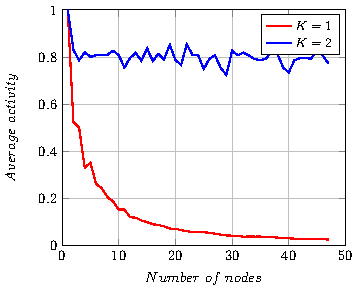
\includegraphics[scale=1.5]{images/K.pdf}
\caption{\emph{Plot of the mean activity of the nodes with network of increasing size.
In the case of $K=1$ (i.e. the mean number of incoming link for each network is one), the mean activity decreases exponentially with the size of the network; in the case of $K=2$ instead, the mean activity of the nodes remains stable with the network size.}}
\label{fig:K}
\end{figure}
In the case of $K=1$, i.e. the mean number of incoming links for each network is one, the mean activity decreases exponentially with the size of the network; in the case of $K=2$ instead, the mean activity of the nodes remains stable with networks of increasing size.
\section{Discrete evolution}
As shown in Chapter \ref{model}, the discrete time evolution of the network is given by the equation:
$$
\sigma_i(t+1)=\Theta\biggl(\sum_jA_{ij}\sigma_j(t)\biggr)
$$
where A is the connectivity matrix of the network.
So this means that each node which has at least one incoming link with a node which is active, in the next step this node will be active.
At each time step we can measure the mean activity of the network, which is the mean number of nodes with the value:
$$
\sigma_i(t) = 1
$$
\section{Control nodes}

\section{Noise}
The second thing to evaluate is the effect of the noise on the evolution of the network and the difference between noise and parametric noise, where parametric noise refers to the noise which infers in the links and not on the nodes.
To add noise to the system, during the discrete evolution of the network, at each time step there is a probability $p$ for the node or for the link to be turned off.
In Figure \ref{fig: noise} we can see the behavior of the mean activity of the network depending on the amount of noise added.
\begin{figure}[h]
\centering
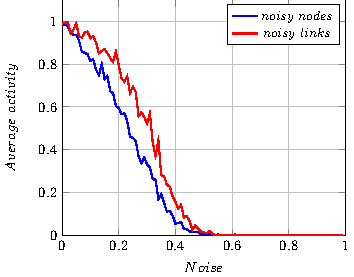
\includegraphics[scale=1.5]{images/noise.pdf}
\caption{\emph{Plot of the effect of the noise on the mean activity on the network. In blue the noise works on the nodes on the network, while in red the noise works on the links.}}
\label{fig:noise}
\end{figure}
